\documentclass[11pt,a4paper]{jarticle}
\usepackage[top=30truemm,bottom=30truemm,left=30truemm,right=20truemm]{geometry}
\usepackage[dvipdfmx]{graphicx}
\usepackage{amsmath,amssymb}
\usepackage{here}
\makeatletter

\def\thefigure{\thesection.\arabic{figure}}
\@addtoreset{figure}{section}
\@addtoreset{equation}{section}
\def\theequation{\thesection.\arabic{equation}}

\def\teach#1{\def\@teach{#1}}
\def\id#1{\def\@id{#1}}
\def\department#1{\def\@department{#1}}

\def\maketitle{
\thispagestyle{empty}
\begin{flushright}
{\Large \@date \par}        % 提出年月日部分
{\Large \@author \par}      % 氏名 
\end{flushright}
\begin{center}
{\Large \@title \par}       % 論文のタイトル部分
\end{center}
\par\vskip 1.5em
}
\makeatother

\title{{\normalsize 東京農工大学 工学府 情報工学専攻 2018年度 修士2年 中間発表}\\ 手指使用量の常時計測のためのウェアラブルデバイスの開発}
\author{{\normalsize 近藤研究室 17646137 松本 崇斗}}
\date{{\normalsize 2018/09/28}}

\begin{document}
\maketitle
1
\newpage

\section{方法}
\subsection{原理}
本研究の手指使用量の測定手法は,指の関節角度の変化が,指の使用量を反映するという仮定に基づく.関節角度の変化の推定には,ウェアラブルデバイスに搭載された赤外線距離センサを用いる.本デバイスは指の基節に装着して使用し,赤外線距離センサで,デバイスから中節までの距離を常時計測する.式2.1の関数を用い,測定された距離を指の関節角度に変換し,指の使用量を測る.距離を角度変換する模式図を図\ref{angle}に示す.

\begin{figure}[H]
\begin{center}
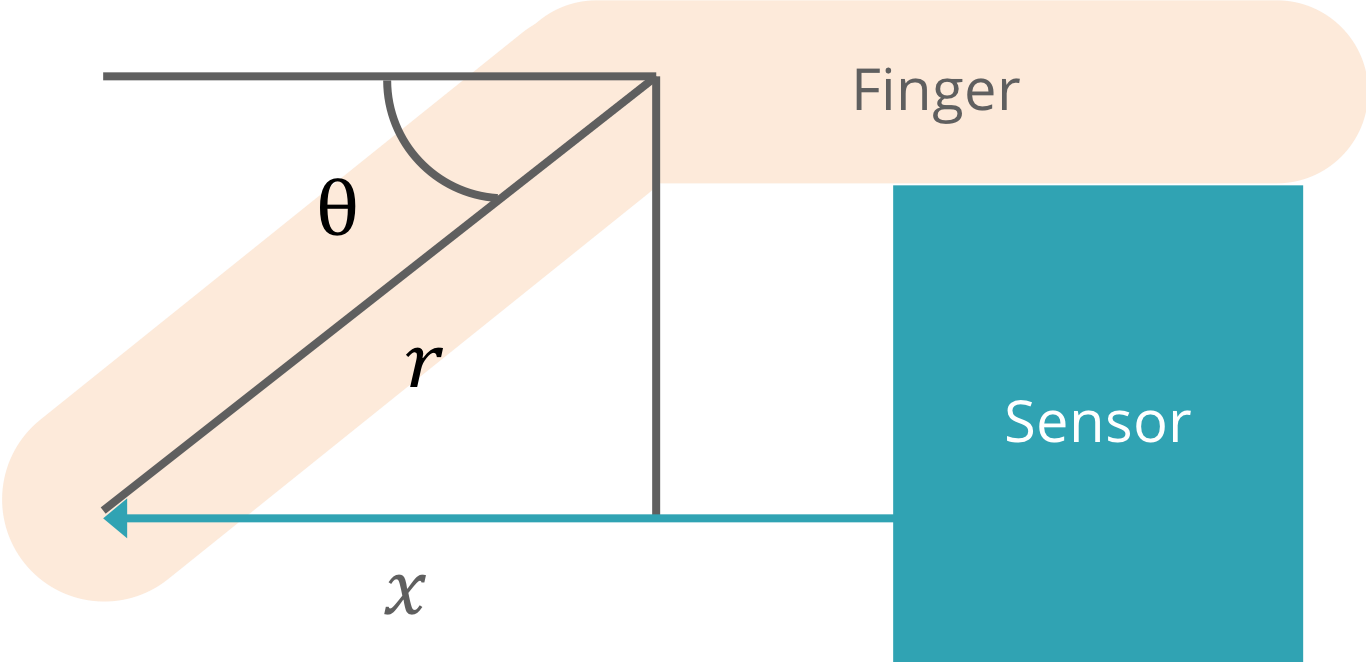
\includegraphics[width=10cm]{fig/principle.png}
\caption{関節角度推定原理}
\label{angle}
\end{center}
\end{figure}

\begin{equation}
\theta = \cos^{-1} \frac{x}{r}
\end{equation}

ここで,$r$は第二関節から指先までの長さ,$x$は屈曲時からの変化距離,$\theta$は伸展時からの変化角度である.

\subsection{ハードウェア}
本デバイスはLED(Osram SFH4550)とフォトトランジスタセンサ(Honeywell SD5410)で構成された赤外線距離センサを用いた指輪型のセンシング部と,手首に取り付けるデータ記録部から成るウェアラブルデバイスである.試作品を図\ref{fig:device}に示す.データ記録のため,マイコン基盤(Adafruit Faether M0)と32GBのSDcardを使用する.また,デバイスの電源として3.7V,900mAhのリポバッテリーを利用し,これにより24時間以上の電源供給が可能である.
\begin{figure}[H]
  \begin{center}
    \begin{tabular}{c}

      % 1
      \begin{minipage}{0.5\hsize}
        \begin{center}
          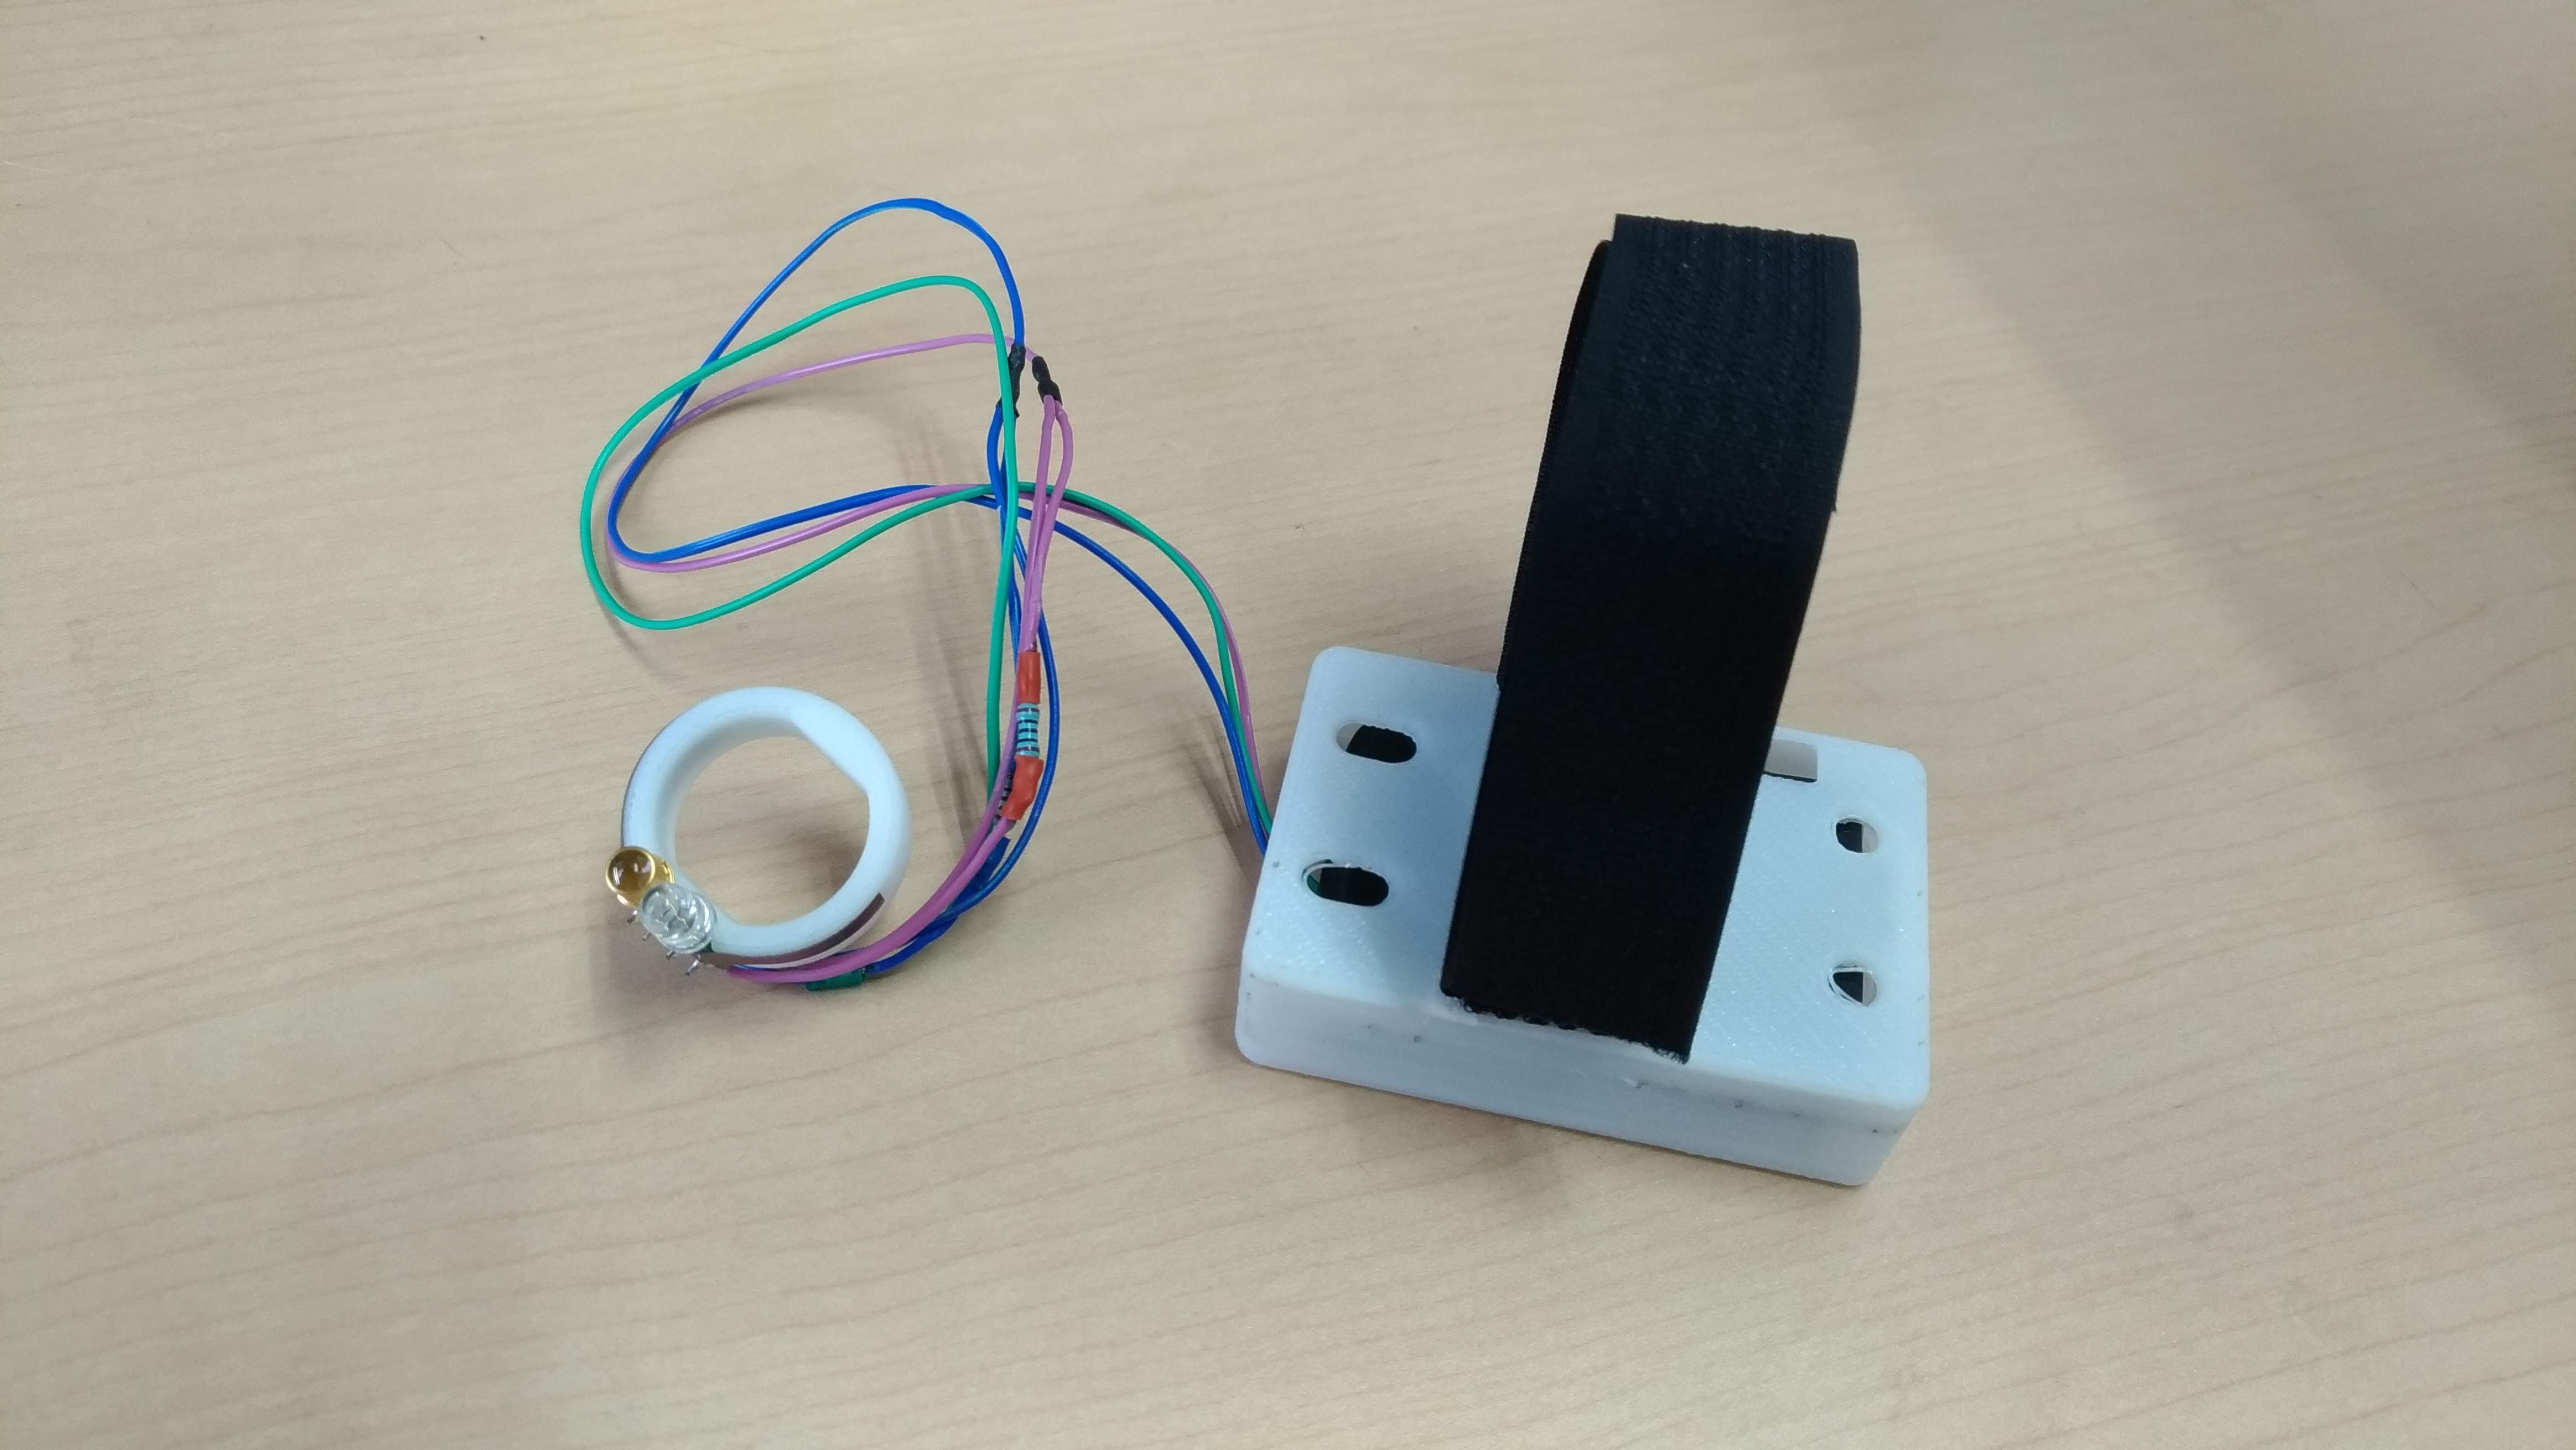
\includegraphics[clip, width=7cm]{fig/fal1.jpg}
          \hspace{3.2cm} [1]外観
        \end{center}
      \end{minipage}

      % 2
      \begin{minipage}{0.5\hsize}
        \begin{center}
          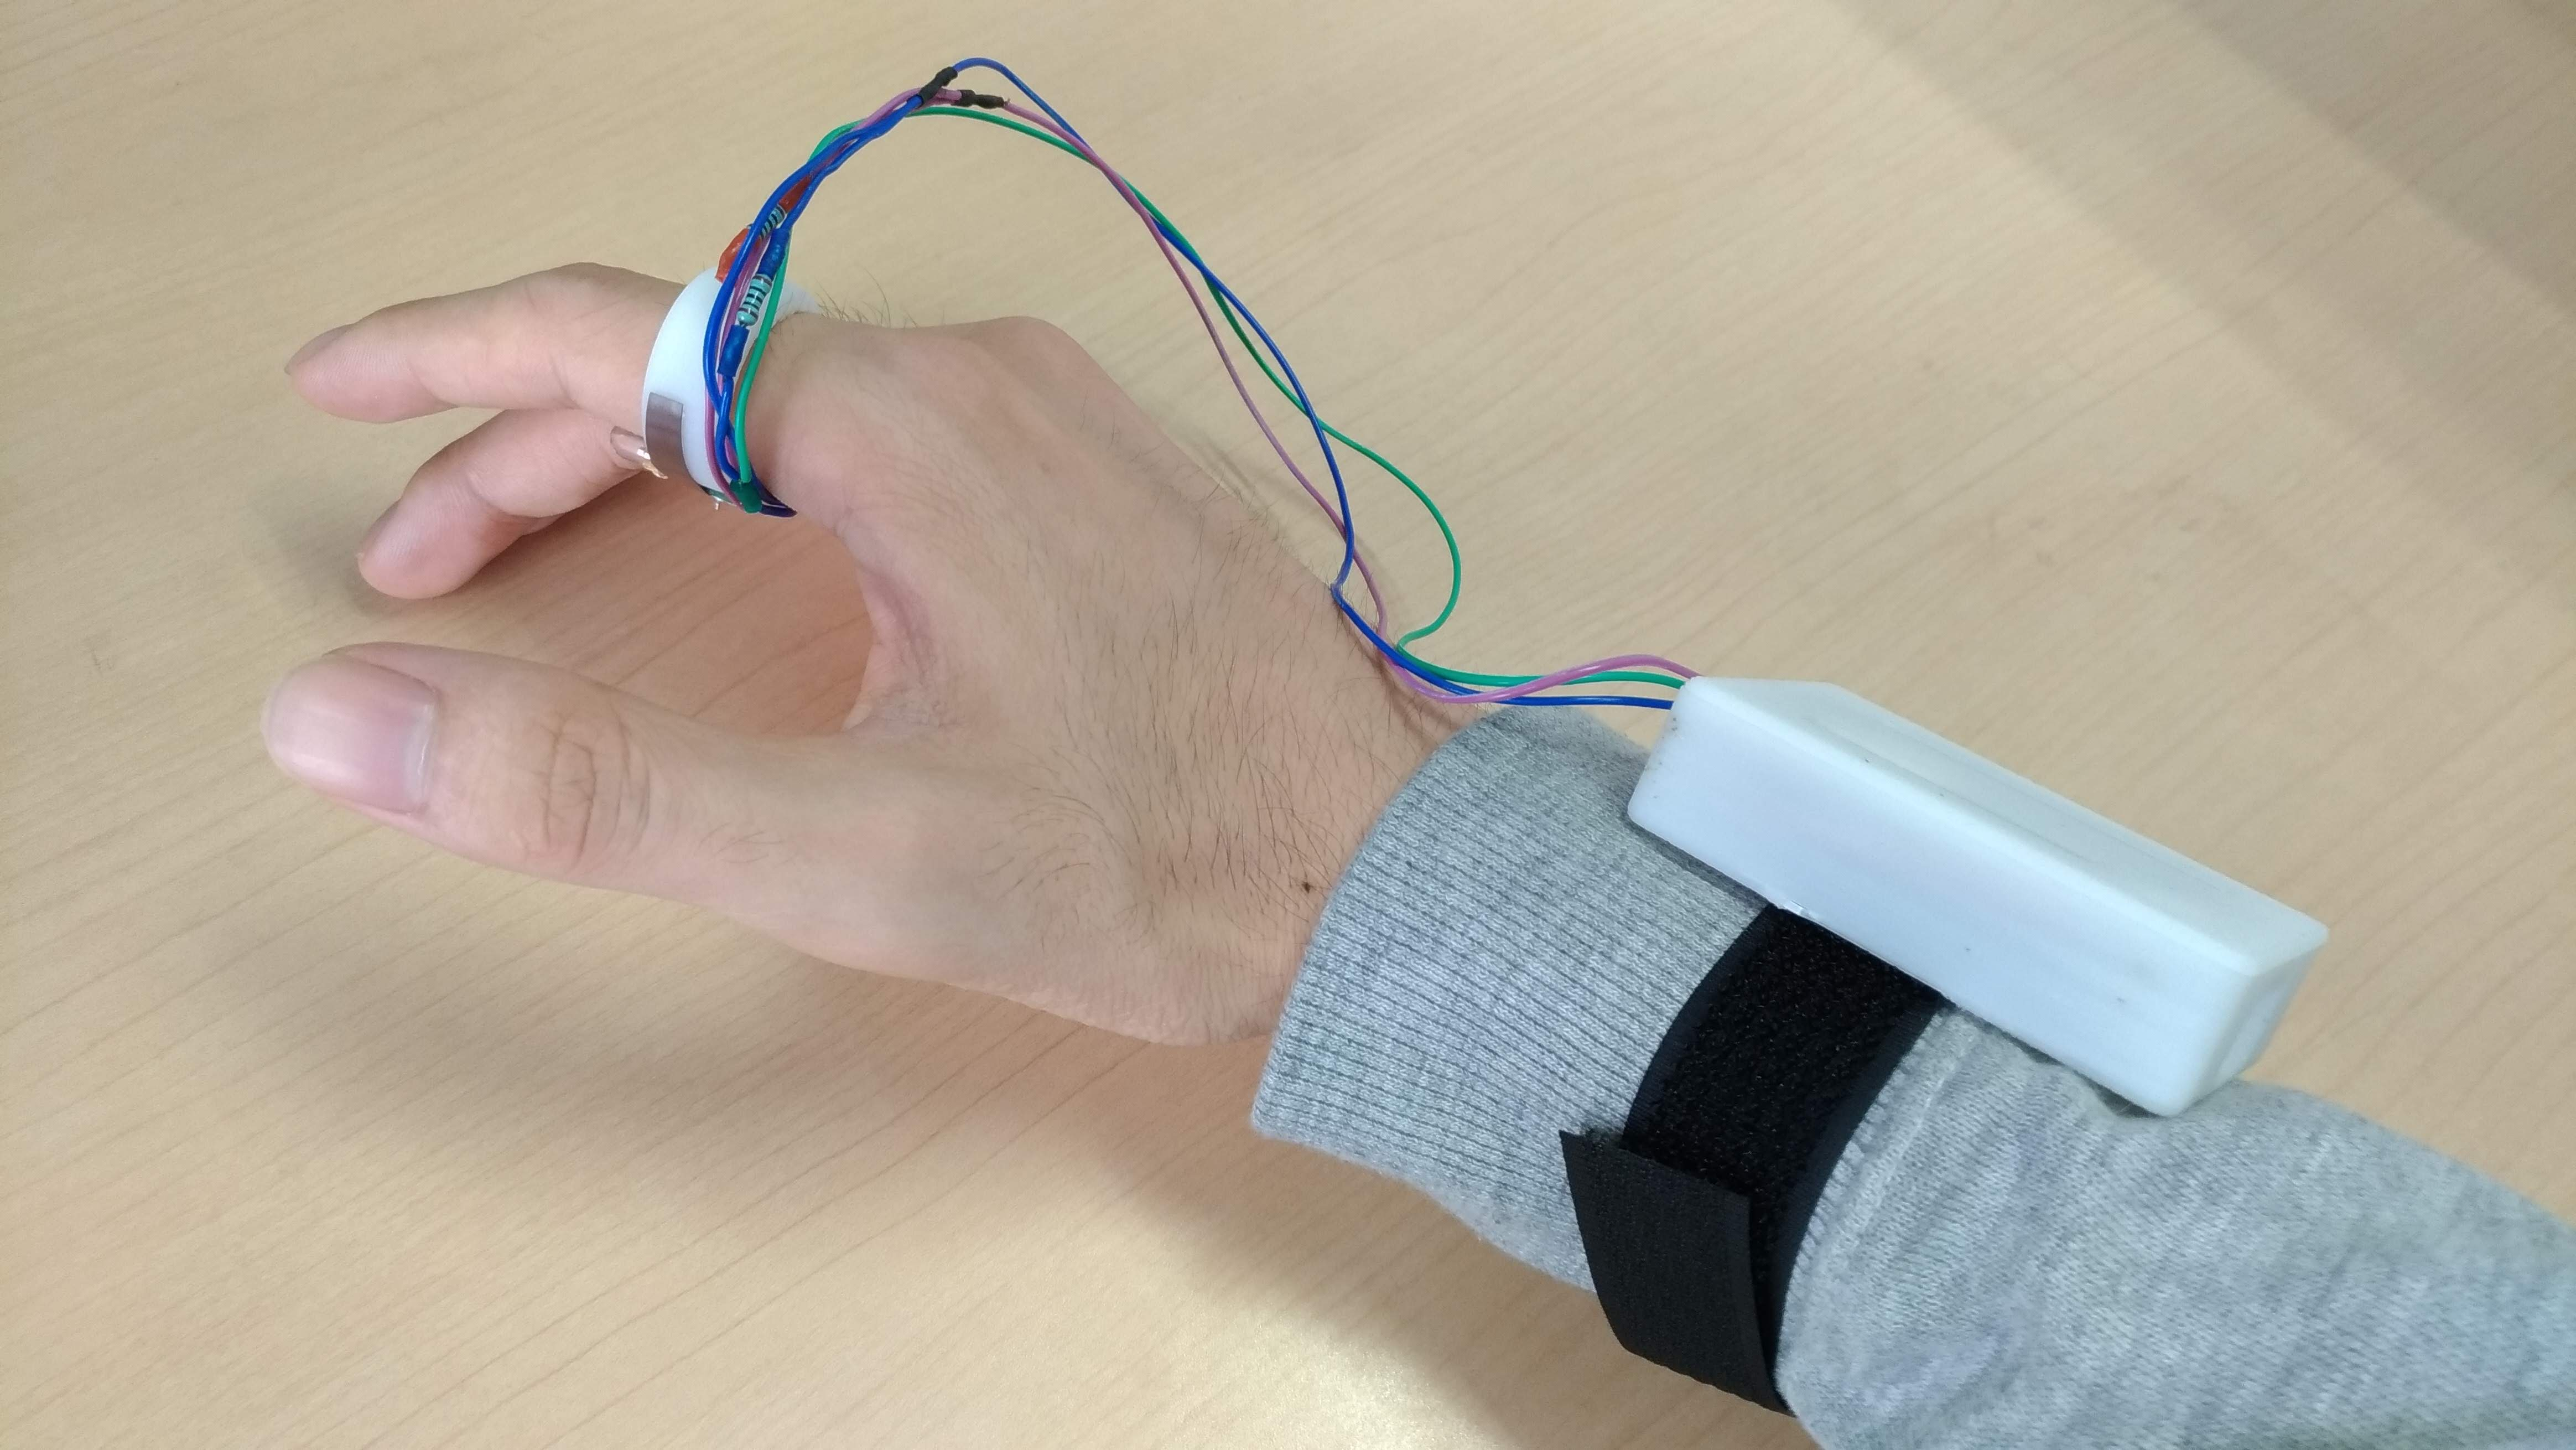
\includegraphics[clip, width=7cm]{fig/fal2.jpg}
          \hspace{3.2cm} [2]装着時
        \end{center}
      \end{minipage}

    \end{tabular}
    \caption{試作したウェアラブルデバイス}
    \label{fig:device}
  \end{center}
\end{figure}

本デバイスの指輪型の装着部分及び,バッテリーとマイコン基盤を収納するためのケースを3DCAD(Fusion 360)で設計し,3Dプリンタ(Dimension 1200es)で印刷し作成した.また,装着時のセンサーのズレによる影響を小さくするために,指輪部分の試作を複数回行なった.指輪部分の3DCAD図を図\ref{fig:ring}にケースの3DCAD図を図\ref{fig:case}に示す.

\begin{figure}[H]
  \begin{center}
    \begin{tabular}{c}

      % 1
      \begin{minipage}{0.25\hsize}
        \begin{center}
          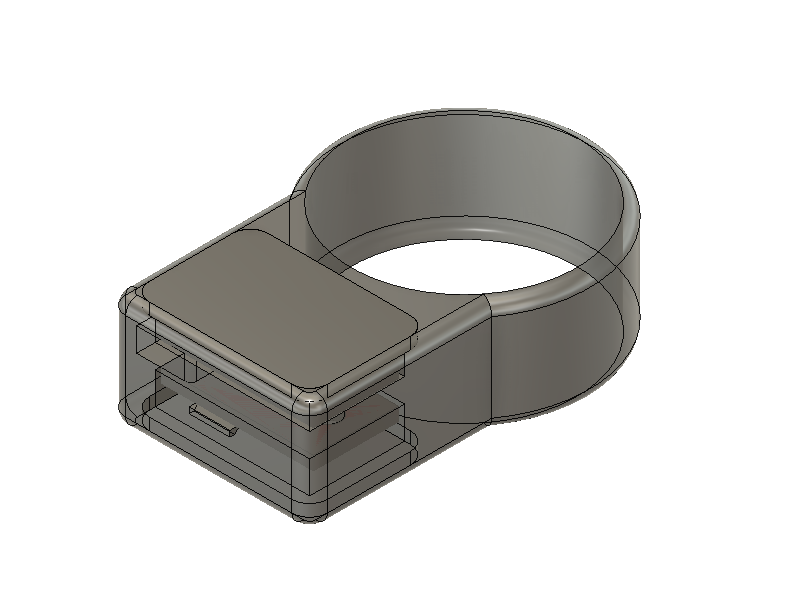
\includegraphics[clip, width=4cm]{fig/ring1.png}
          \hspace{3.2cm} [1]第一試作
        \end{center}
      \end{minipage}

      % 2
      \begin{minipage}{0.25\hsize}
        \begin{center}
          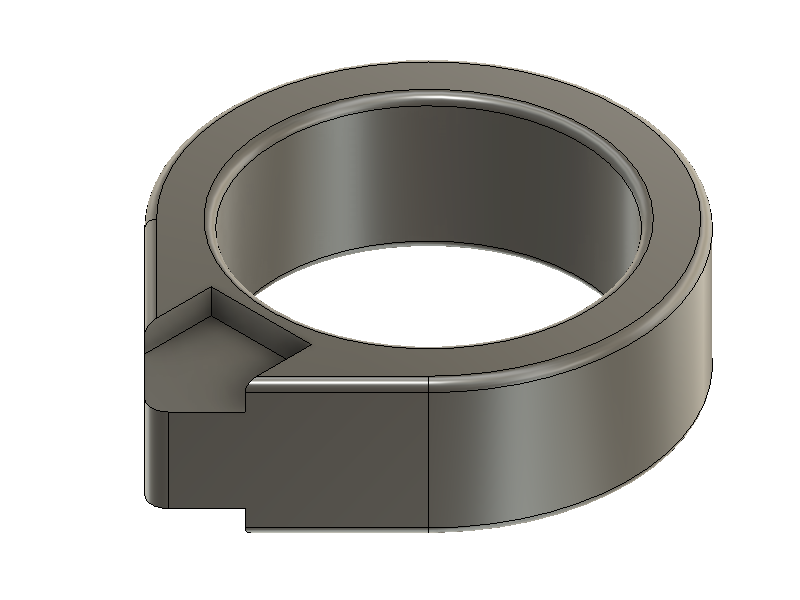
\includegraphics[clip, width=4cm]{fig/ring2.png}
          \hspace{3.2cm} [2]第二試作
        \end{center}
      \end{minipage}

            \begin{minipage}{0.25\hsize}
        \begin{center}
          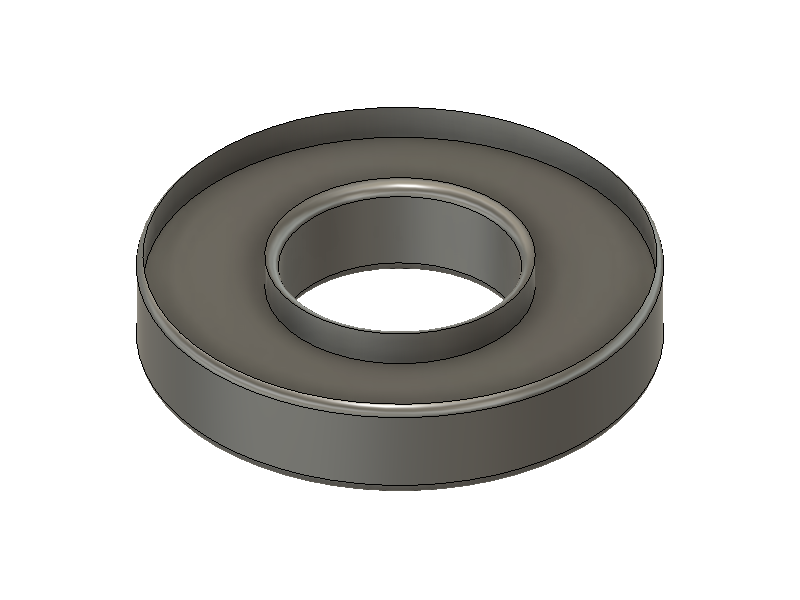
\includegraphics[clip, width=4cm]{fig/ring3.png}
          \hspace{3.2cm} [3]第三試作
        \end{center}
      \end{minipage}

            \begin{minipage}{0.25\hsize}
        \begin{center}
          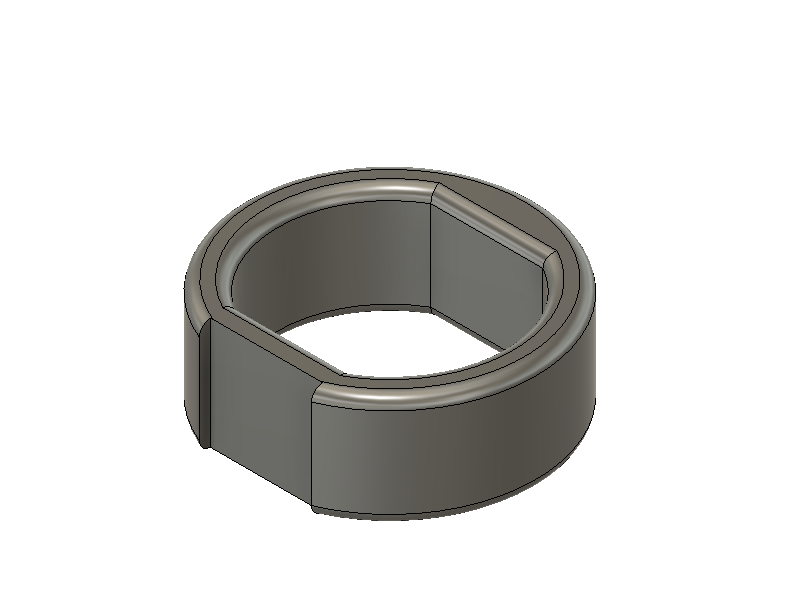
\includegraphics[clip, width=4cm]{fig/ring4.png}
          \hspace{3.2cm} [4]第四試作
        \end{center}
      \end{minipage}


    \end{tabular}
    \caption{指輪部分の3DCAD図}
    \label{fig:ring}
  \end{center}
\end{figure}

複数の試作の内,図\ref{fig:ring}[4]の3DCAD設計を本デバイスに採用した.


\begin{figure}[H]
  \begin{center}
    \begin{tabular}{c}

      % 1
      \begin{minipage}{0.5\hsize}
        \begin{center}
          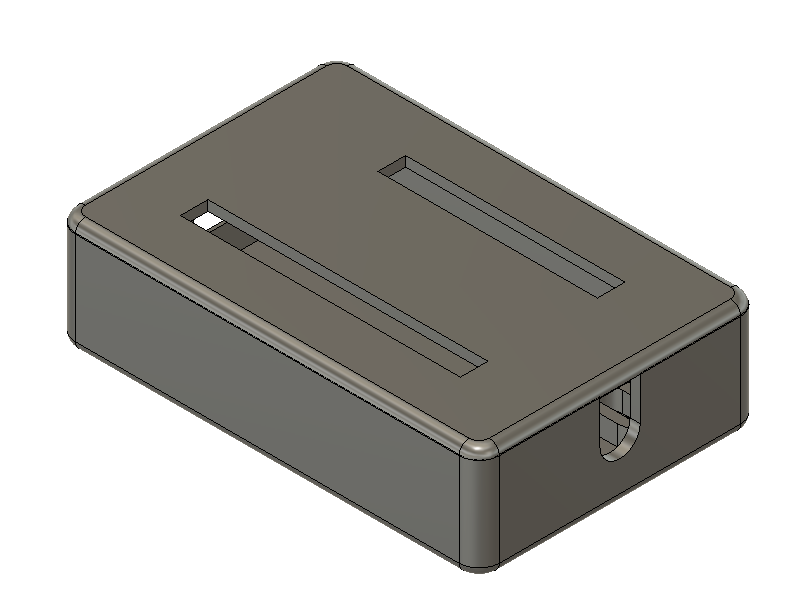
\includegraphics[clip, width=6cm]{fig/case1.png}
          \hspace{3.2cm} [1]天板あり
        \end{center}
      \end{minipage}

      % 2
      \begin{minipage}{0.5\hsize}
        \begin{center}
          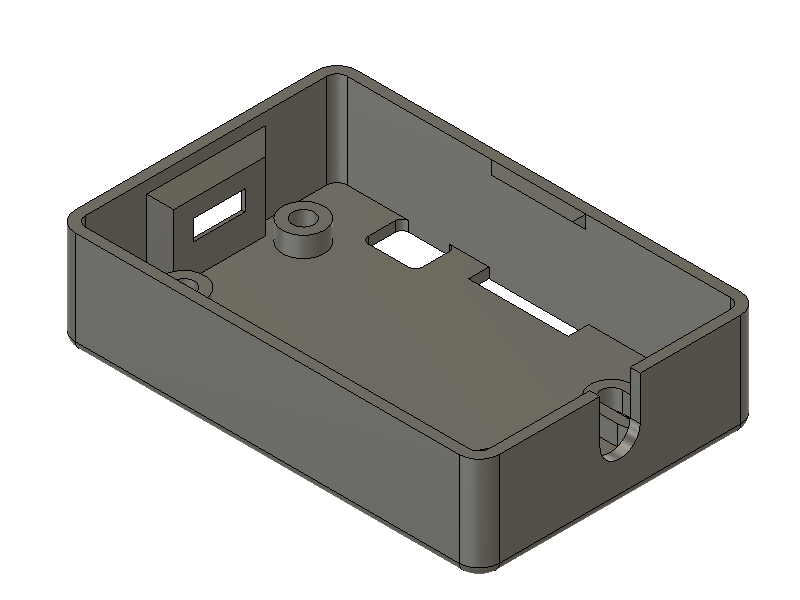
\includegraphics[clip, width=6cm]{fig/case2.png}
          \hspace{3.2cm} [2]天板なし
        \end{center}
      \end{minipage}


    \end{tabular}
    \caption{ケース部分の3DCAD図}
    \label{fig:case}
  \end{center}
\end{figure}


\subsection{キャリブレーション}
赤外線距離センサは物体に反射し,フォトトランジスタで受光した赤外線の強さを計測することで,距離を計測する.
しかし,同じ距離であっても赤外線が反射する物体によっては,違う
受光量となる場合がある.これは物体によって光の反射率が違い,同じ距離でも,フォトトランジスタで受け取る受光量が違ってくるためである.つまり,人によって,指の長さや皮膚の色が違うため,同じセンサ値であっても,本来の距離が変わってくる問題がある.この問題を解決するために,被験者毎に皮膚の反射率を調べることが望ましいが,本システムは日常生活での使用を目的としており,キャリブレーション自体が簡単であることが求められる.
そのため,本システムでは計測される距離と受光量の関係を求め,簡単にキャリブレーションが可能な方法を提案する.キャリブレーションには以下の3つのパラメータを用いる.

\begin{itemize}
 \item デバイスを装着する指の長さ
 \item 指伸展時のセンサ情報
 \item 指屈曲時のセンサ情報
\end{itemize}


\section{結果}
\subsection{予備実験: ジェスチャ識別}
予備実験として健常者を対象に,本システムのジェスチャの認識精度を調査した.この実験の際は,LED(Osram SFH4550)とフォトトランジスタセンサ(Honeywell SD5410)の代わりに,赤外線距離センサ(qtr-1a)を2つ使用し,図\ref{sensor}の位置に取り付けた.
\begin{figure}[H]
\begin{center}
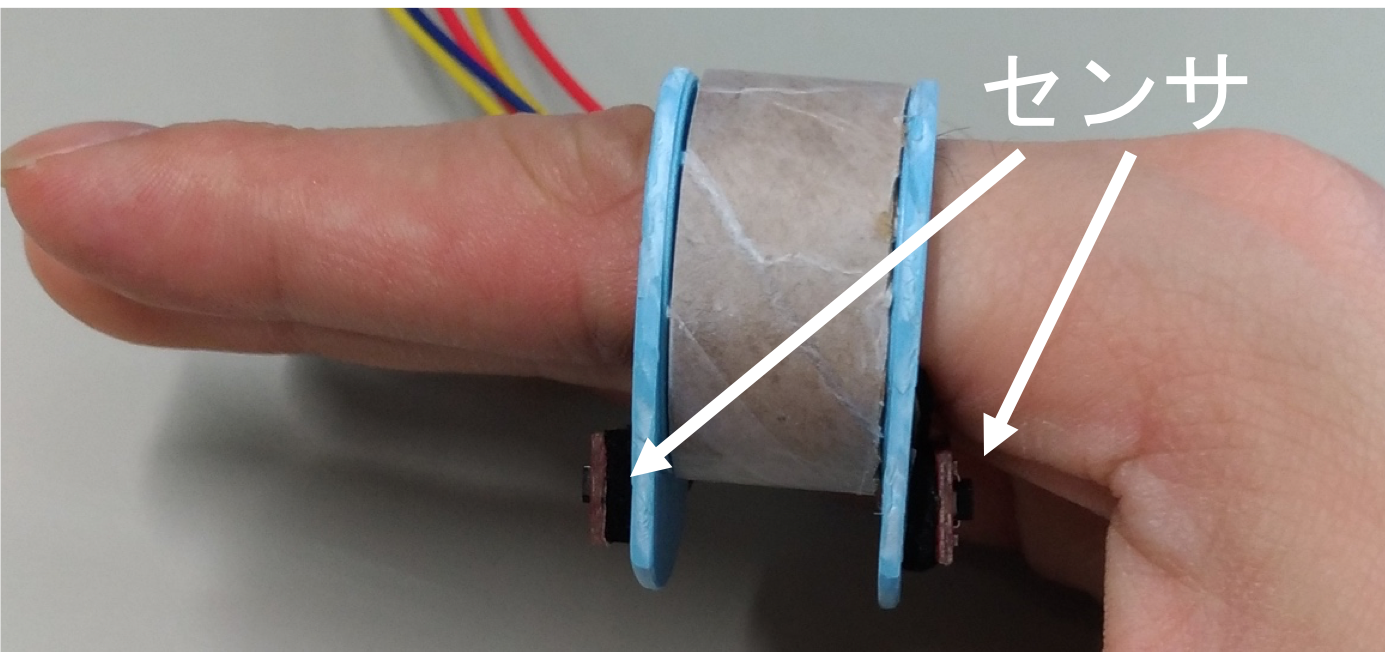
\includegraphics[width=10cm]{fig/sens1.png}
\caption{センサ取り付け位置}
\label{sensor}
\end{center}
\end{figure}

手指を閉じた状態,開いた状態,示指と母指で輪を作った状態,計3つのジェスチャを指示し被験者に行ってもらった.ジェスチャの種類を図\ref{gesture}に示す.被験者は椅子に座った状態で,本デバイスを装着した手でジェスチャを行った.一つのジェスチャを5秒間保持してもらい,その時のセンサーデータを収集した.5秒間のセンサーデータを時間で平均したセンサ値をジェスチャ識別のために利用した.
また,センサデータは各ジェスチャにつき60回記録し,五人の被験者センサデータを収集した.センシングの際のサンプルレートは100Hzとした.
合計で一人につき180データ(60データ$\times$3ジェスチャ)を収集した.

\begin{figure}[H]
\begin{center}
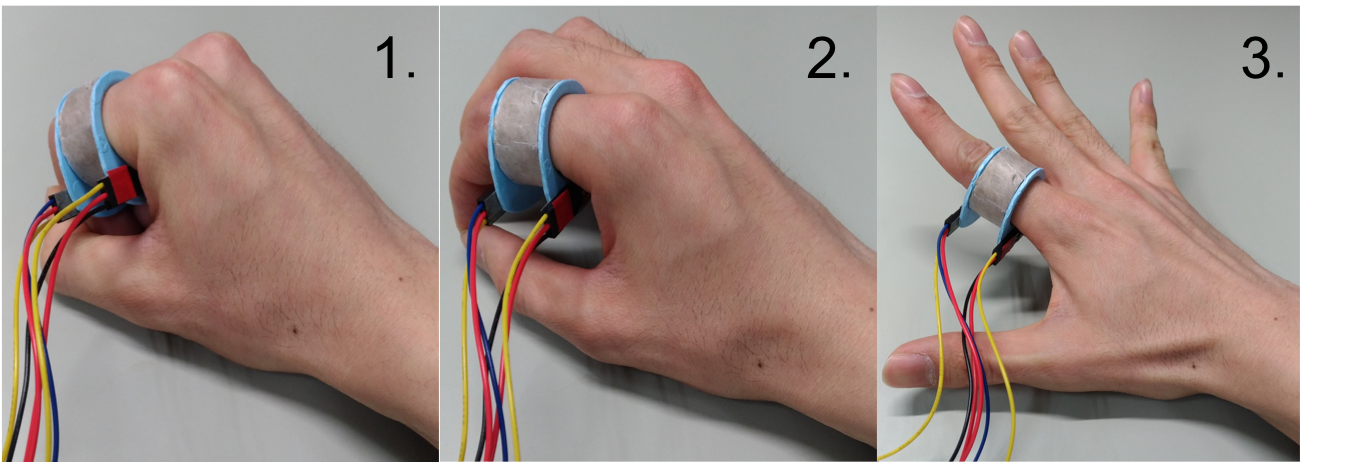
\includegraphics[width=10cm]{fig/gesture.png}
\caption{ジェスチャの種類}
\label{gesture}
\end{center}
\end{figure}


3つのジェスチャを識別するため,1対1分類法,線形Support Vector Machineを用いた.5人すべて,900データ(180データ$\times$5人)をジェスチャごとにラベル分けし,ジェスチャ識別に利用した.これらのデータの内,各ラベルに対し,データの80\%をトレーニングデータ,20\%をテストデータとした.

\begin{figure}[H]
\begin{center}
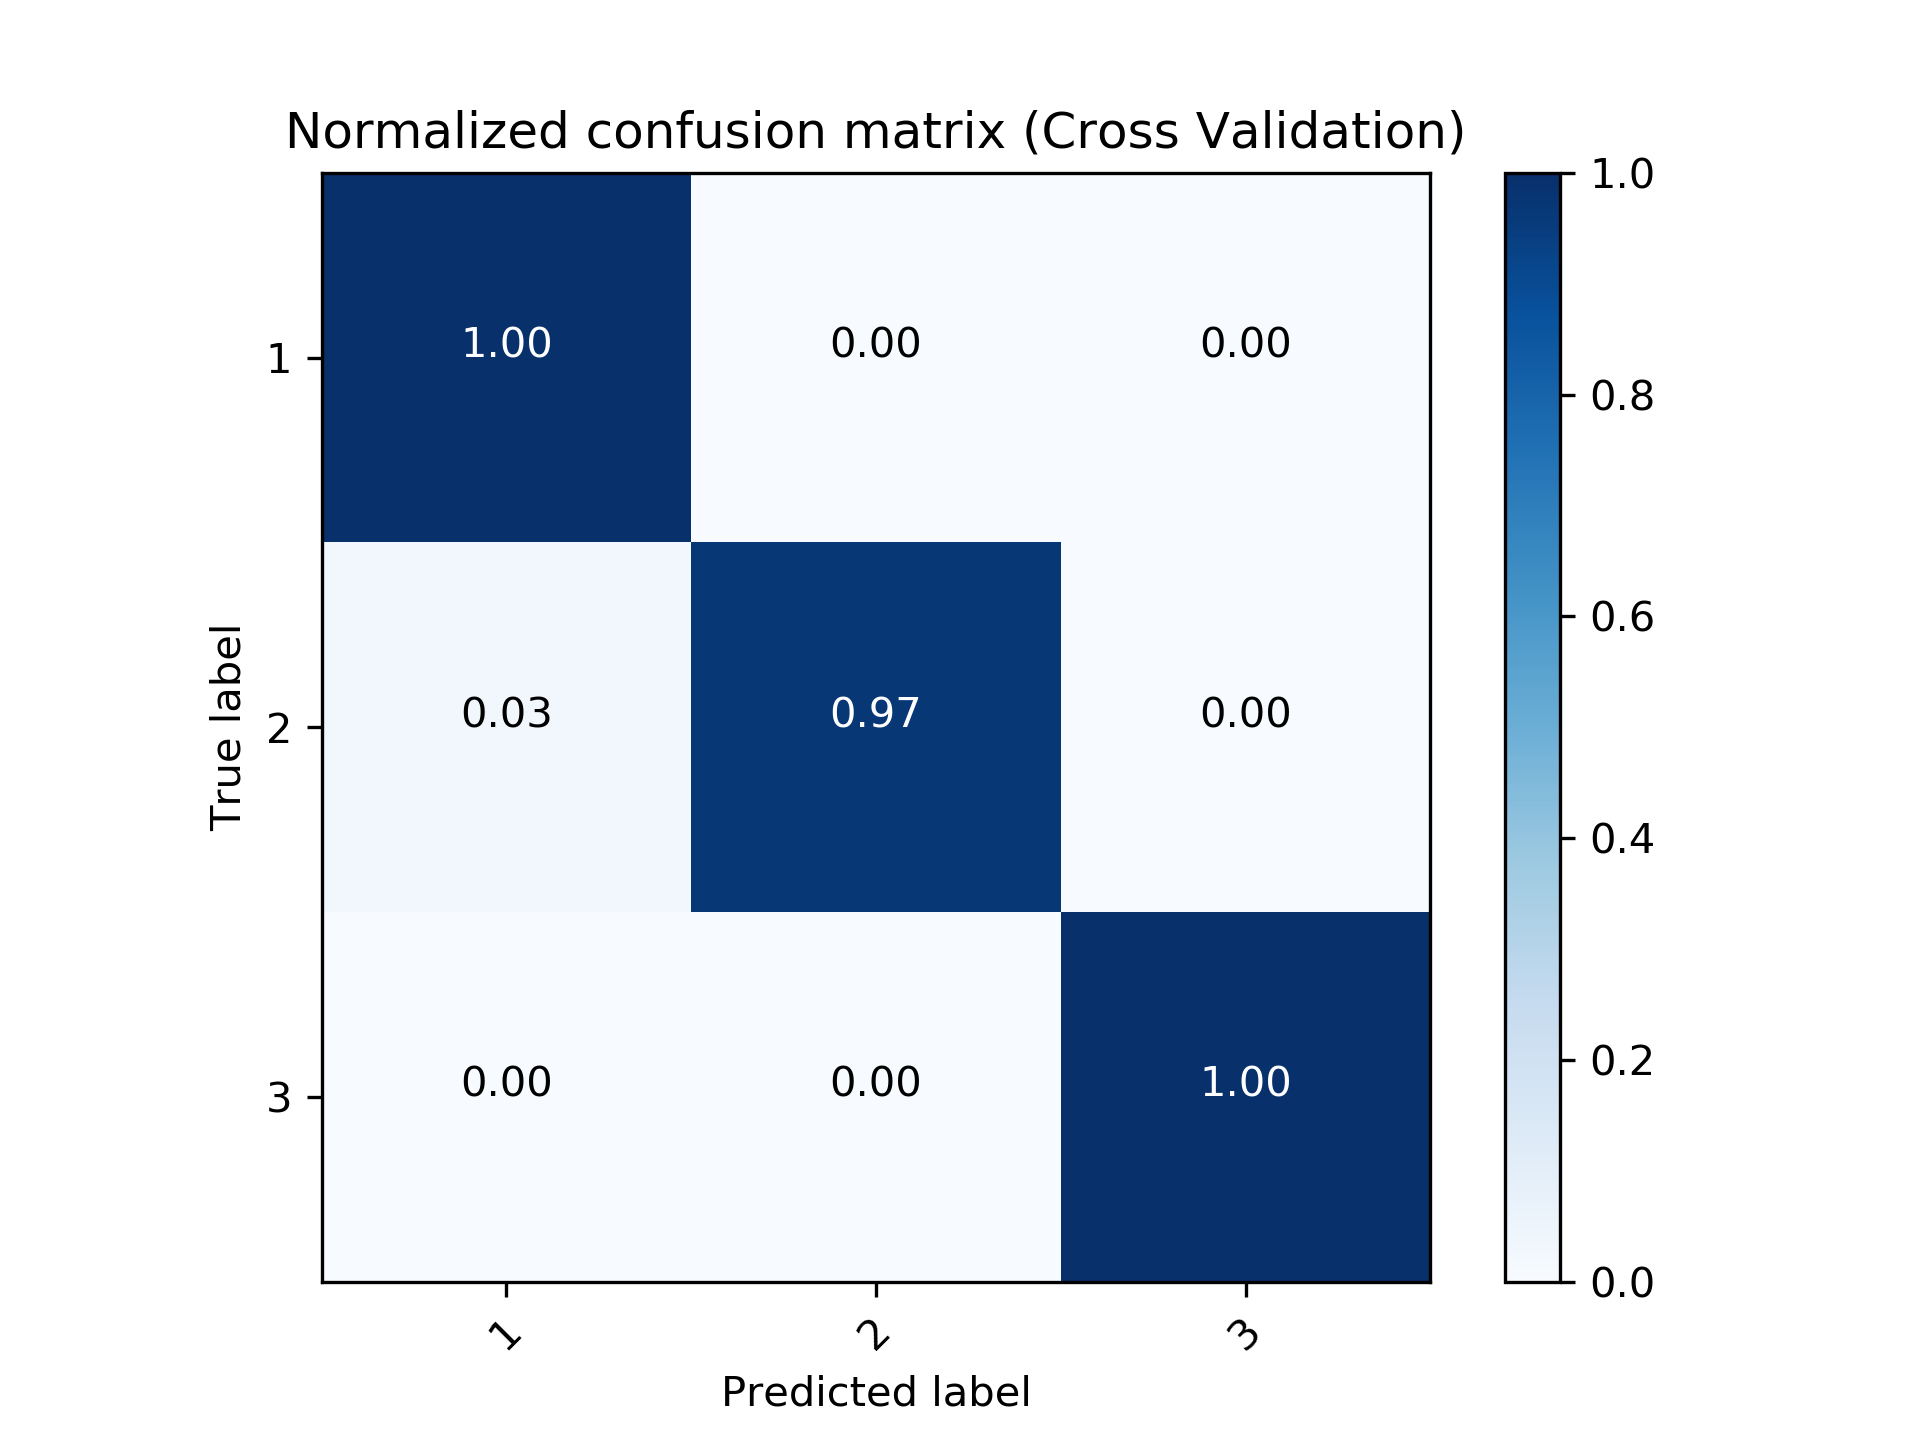
\includegraphics[width=10cm]{fig/confusion_matrix.png}
\caption{全ての被験者のデータを5分割交差検証した結果}
\label{matrix}
\end{center}
\end{figure}


図\ref{matrix}より,ジェスチャ1と3を100\%の正解率で認識することが可能であることが分かった.5分割交差検証を行った結果,ジェスチャの平均正解率は98.9\%,分散3.9\%であった.結果から本手法により3つのジェスチャの識別が可能であることが示唆された.

\subsection{関節角度推定(予定)}
本システムによって推定された関節角度の精度を調査する.
被験者の第二指に本デバイスを装着し,ピンチインとピンチアウトをそれぞれ10回ずつ行ってもらう.計測時間は1セット30秒間で,センサのサンプルレートは10Hzとする.
以上の条件のもと,一人の被験者に10セットタスクを行なってもらう.その時,関節角度の正解データとして,OpenCVのカラーマーカーを用いた関節角度の計測を行う.また,精度の評価にはMean Absolute Error(MAE)を用いる.
\begin{equation}
MAE = \frac{1}{n} \sum^n_{k=1} |f_i-y_i|
\end{equation}
ここで$f_i$と$y_i$はそれぞれ時間$i$のときの本システムによる推定関節角度とOpenCVによる関節角度の計測値である.


\section{修士論文構成案}
以下に修士論文文章構成案を示す.\\
\noindent
第1章 序論\\
\hspace{0.5cm}1.1 背景\\
\hspace{0.5cm}1.3 先行研究の紹介\\
\hspace{0.5cm}1.2 論文の構成\\
第2章 原理\\
\hspace{0.5cm}2.2 本研究の目的\\
第3章 実験設定\\
第4章 実験結果\\
第5章 考察\\
第6章 まとめ\\
\hspace{0.5cm}6.1 まとめ\\
\hspace{0.5cm}6.2 今後の展望\\
謝辞\\
参考文献\\


\bibliographystyle{jplain}
\bibliography{library}
\end{document}